\section {INOVAÇÃO ABERTA}
\label{inovacaoaberta}

Como citado anteriormente, a Inovação Aberta é um  conceito criado por Henry Chesbrough que versa a respeito da criação de inovações com a possibilidade da participação de atores externos. Ele trata deste tema em seu livro “Inovação Aberta” (\citeyear{chesbrough2003}) como um novo paradigma de inovação.

O conceito é descrito como a concentração de uso de conhecimento externo e/ou exportação do conhecimento interno visando a potencialização dos processos inovativos, num processo o qual se torna benéfico para ambas as organizações envolvidas.

\citeauthor{chesbrough2003} (\citeyear{chesbrough2003}) mostra no gráfico abaixo como ocorre o processo inovativo nas organizações através do método de inovação fechada, por meio do cenário de conhecimento afunilado, que demonstra as limitações da mesma. Apesar de existirem muitas ideias de inovações (representada aqui pelos \textit{inputs}), poucas delas são utilizadas e/ou aproveitadas.

O panorama se torna empobrecido, pois ambas as companhias possuem diversas ideias, mas nem todas são usadas, e elas poderiam ser aproveitadas uma pela outra, tanto para potencializar suas próprias ideias, quanto para potencializar as ideias da outra organização.

\begin{figure}[H]
    \caption{O cenário do conhecimento na inovação fechada}
    \centering
    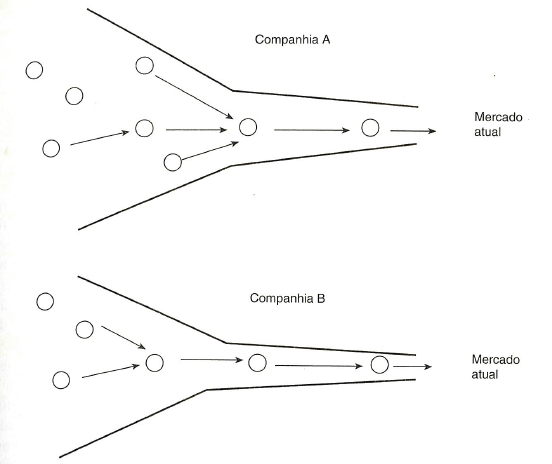
\includegraphics[width=\linewidth]{images/fundamentacao/inovacaofechadachesbrough.png}
    \label{fig:inovacaofechada}
    
    Fonte: \citeauthor{chesbrough2003} (\citeyear{chesbrough2003}, p. 47).
\end{figure}

Existe também uma classificação da forma de realizar a inovação aberta, trazidos em \textit{“Novas Fronteiras em Inovação Aberta”} de \citeauthor{chesbrough2014} (\citeyear{chesbrough2014}, p. 43-45):

\begin{figure}[H]
    \caption{Modelo de inovação aberta}
    \centering
    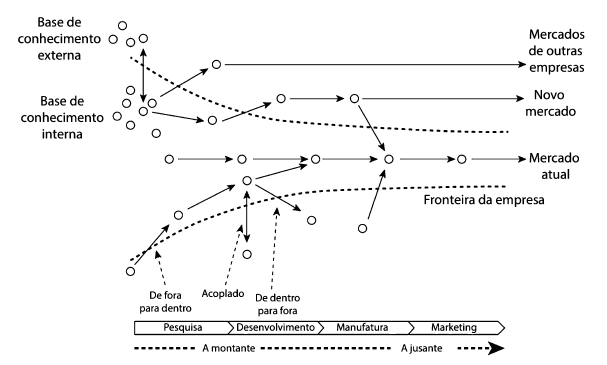
\includegraphics[width=\linewidth]{images/fundamentacao/modeloinovacaoaberta.png}
    \label{fig:modeloinovacaoaberta}
    
    Fonte: \citeauthor{chesbrough2014}(\citeyear{chesbrough2014}, p. 43).
\end{figure}

\begin{itemize}
    \item \textbf{Inovação de dentro para fora} (\textit{Outside-in} ou \textit{Inbound}): esse modelo envolve a abertura do processo de uma organização para outras organizações e atores externos, servindo como ideias e entradas para outras organizações. Também é utilizado estrategicamente para monetização mediante licenciamento ou venda de propriedade intelectual, onde a empresa pode disponibilizar alguma inovação que não faz parte do escopo da organização, ou na qual a mesma não possui mais interesse, dentre outras situações.

    \item \textbf{Inovação de fora para dentro} (\textit{Inside-out} ou \textit{Outbound}): é o tipo mais estudado de inovação aberta, que consiste no processo de inovação da organização aberto a entradas e contribuições de atores externos, por meio de ideias, conhecimentos, parcerias, aquisições e outros.

    \item \begin{sloppypar}
    \textbf{Inovação acoplada} (\textit{Coupled}): segundo \citeauthor{chesbrough2014} (\citeyear{chesbrough2014}, p.~42), esse modelo foi proposto por Gasmann e Enkel, sendo o resultante da combinação dos fluxos de inovação de dentro para fora e de fora para dentro, entre os atores do processo. Pode envolver de dois a mais atores, via \textit{joint\-ventures}, consórcios, ecossistemas, dentre outros. Essa inovação acoplada pode acontecer de duas formas:
        \begin{itemize}
            \item Bidirecional: cada um dos atores realiza isoladamente seus processos inovativos e criativos, e em seguida compartilham entre si os conhecimentos gerados nesse processo.
            \item Interativa: essa forma acontece através da cocriação, onde os atores constroem o processo inovativo e criativo colaborativamente, não ocorrendo isoladamente dentro de cada organização, mas sim em um ambiente “externo” com a presença das duas organizações, como mostrado na figura abaixo:
            \begin{figure}[H]
    \caption{Duas formas de inovação aberta acoplada}
    \centering
    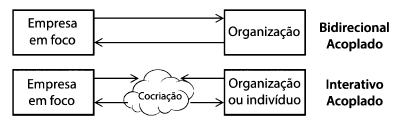
\includegraphics[width=\linewidth]{images/fundamentacao/cocriacao.png}
    \label{fig:cocriacao}
    
    Fonte: \citeauthor{chesbrough2014} (\citeyear{chesbrough2014}, p. 43).
\end{figure}
        \end{itemize}
    \end{sloppypar}
\end{itemize}


Um estudo investigando a realização da Inovação Aberta em grandes organizações, realizado por Sabine Brunswicker e Henry Chesbrough, denominado \textit{“The Adoption of Open Innovation in Large Firms”} também trouxe uma grande colaboração para a Inovação Aberta, por meio de práticas para o gerenciamento destas inovações, via \textbf{Modos de governança} \cite{brunswicker2018}:
\begin{itemize}
        \item \textbf{Comunidades e redes profissionais}: os colaboradores da organização participam de comunidades abertas, onde seus membros colaboram e compartilham o conhecimento em prol da comunidade, com regras da comunidade;
        \item \textbf{Comunidades de Inovação Aberta patrocinadas por empresas}: a organização convida atores externos a participar dos processos inovativos da mesma, com regras da organização;
        \item \textbf{Rede informal}: Funcionários da organização praticando \textit{networking} em conferências, eventos e afins, de modo a acessar conhecimento externo à organização;
        \item \textbf{Intermediários de Inovação Aberta}: organizações contratam empresas especializadas em Inovação Aberta para buscar soluções para seus problemas em potencial. Essas organizações especializadas competem entre si;
        \item \textbf{Concursos e torneios de Inovação}: participantes convidados a oferecer soluções inovativas em processos competitivos, em vez de colaborativos, recompensados financeiramente e/o de outras formas;
        \item \textbf{Parcerias bilaterais}: as duas partes interessadas cocriam uma solução inovativa para um problema, através da troca mútua de conhecimento, através da relação de confiança;
        \item \textbf{Contratos bilaterais}: as duas partes interessadas realizam um contrato para troca de conhecimento, por meio de estruturas formais de compartilhamento de conhecimento, como licenciamento de direitos de propriedade intelectual, patentes, entre outros.
\end{itemize}
